\section{Quantum Computational Complexity}\label{chap:complexity}
The theory of computational complexity centres around the question what the minimal required resources to solve a given computational problem are. Although one can discuss about different resources, time, space, energy, let us focus here on the specific question of (run)time required to solve a given problem.

Summing up two n-bit numbes takes $O(n)$, while mutiplication takes in principle $O(n \log n)$. Search in a structured data base takes $O(\log n)$.
\footnote{We say the function $f(n)$ is in the class of functions $O(g(n))$ if at some point the function $g(n)$ scaled by an arbitrary constant grows faster than $f(n)$. Formally this can be defined as
\begin{align*}
    O(g(n)) = \left\{f(n) \;|\; \exists n_0\in\mathbb{N}, \forall c\in\mathbb{N}, \forall n\geq n_0: f(n)\leq c\cdot g(n)\right\}
\end{align*}
we will however not need the formal definition. }
The big-O is essentially the ``smaller as'' for functions, meaning $f\in O(g)$ can be read as ``$f$ is asymptotically smaller than $g$''.~\footnote{in the same way we have $f\in \Omega(g)$ for $f$ larger $g$ and $f\in\Theta(g)$ for $f$ equal $g$} 

We can then classify the problems as tractable problems, which can be solved in polynomial time, and intractable problems, which are superpolynomial -- where superpolynomial just means that a function grows larger than any polynomial. An exponential function is for example superpolynomial (but not all superpolynomial functions are exponential).~\footnote{for this course it is fine to just think about polynomial and exponential though}
To classify tractable problems, the complexity class $\mathrm{P}$ was introduced. \\

The classical complexity classes below are all formally defined for Turing machines -- which you can just view as ``classical computer''.
Here is a very simple example of a Turing machine: consider the problem of determining if a given integer is odd or even, we can call it $\texttt{even}(n)$. We can encode integers in binary, meaning we can use the alphabet $\Sigma=\left\{0,1\right\}$ to form words that represent integers. We can now write the binary representation of any integer onto the tape of a Turing machine and let the machine figure out if the integer is even -- if it is even, the machine will accept. All the machine needs to do, is to move to the end of the input string and check if it is the symbol 0 -- if so, then the machine can accept, otherwise it just halts (or rejects). If the string consists of $O(N)$ symbols, then this takes roughly $O(N)$ elementary transitions for the machine. Therefore the problem is solved in polynomial time on a Turing machine, and we have $\texttt{even}\in \mathrm{P}$. Note here that the choice of a binary alphabet is kind of arbitrary. We could have also used decimal representation with the alphabet $\Sigma=\left\{0,1,2,3,4,5,6,7,8,9\right\}$. Then, the machine needs to move to the last entry of the input and check if it is any of the symbols $0,2,4,6,8$. So, the machine needs to have some more transitions defined, but the actual runtime will stay linear.\\
If we change the encoding of our integer to "least significant bit first" then it will only take a single step for a suitable Turing machine (simply just checking if the first bit is 0). The same is true if we take a Random Access Machine (a different model of computation) that is able to directly access datafields. Since the computers we use are closer to Random Access Machines.

\subsection{Complexity Classes}

Besides the problems that can be solved efficiently, we can also form two more classes, where we don't necessarily know if we can solve efficiently, but where we at least can certainly verify a given solution efficiently.

\begin{def*}[Basic Complexity Classes]\phantom{...}
\begin{align*}
\mathrm{P} &: \text{efficient algorithm}\\
\mathrm{NP}&: \text{efficient verification with short proofs}\\
\mathrm{coNP} &: \text{efficient falsification with short proofs}     
\end{align*}
\end{def*}
Efficient means that there exists an algorithm that runs in polynomial time w.r.t the length of the original instance of the problem. A short proof is an additional input whose length is polynomially bounded by the length of the original instance of the problem.
Here are some examples:\\

$\texttt{SubsetSum}(I,c)$: given natural numbers $I=\left\{n_1,n_2,\dots n_N\right\}$ determine if there is a subset $S\subseteq I$ such that the numbers in $S$ add up to $c$. We have that $\texttt{SubsetSum}\in \mathrm{NP}$ since we can efficiently verify: If the instance is true then a subset $S$ with the requested properties has to exist. If given such a subset $S$ (this is the short proof) it is easy to check if it is a subset of $S$ and the numbers indeed add up to $c$ (this is the verification). On the other hand: It is unclear if we can also easily falsify the problem, meaning if the answer is no, we don't know how to proof that efficiently -- the problem is most likely not in $\mathrm{coNP}$. We also don't know how to solve the problem, and it is most likely not in $\mathrm{P}$.\\

$\texttt{Taut}(\varphi)$: Determine if a given Boolean function is a tautology (meaning if it is constant 1). We have $\texttt{Taut}\in \mathrm{coNP}$ because it is easy to falsify: if the answer is no, it suffices to provide a variable assignment that evaluates to false. On the other hand, we don't know how to verify the problem: if the answer is yes, it is hard to efficiently verify that the function is indeed a tautology. And similarly we don't know how to efficiently decide the problem.\\

\texttt{Factoring}$(n)$: Decompose a given integer $n$ into its prime factors. The decision version is \texttt{Factor}$(n,m)$: Determine if there is a $k\leq m$ that is a factor of $n$. We have $\texttt{Factor}\in \mathrm{NP}$ since we can easily verify (provide the answer and check if it is indeed a factor of $n$). But we also have $\texttt{Factor}\in \mathrm{coNP}$ because we can also easily verify: if there is no factor of $n$ smaller than $m$ we can provide the prime-factorization of $n$ and check that all factors are larger than $m$.~\footnote{non-trivial structure: the fundamental theorem of arithmetic guarantees us that each integer $n$ has a unique factorization using prime numbers. It is also possible to efficiently check if a given number is a prime number (AKS-primality test).}

\begin{def*}[Complete Problems] If a decision problem is complete for a class, it essentially means that all other problems within that class can be efficently transformed into instances of the complete problem. The complete problems in $\mathrm{NP}$ and $\mathrm{coNP}$ form the classes $\mathrm{NPC}$ and $\mathrm{coNPC}$. Examples (without proofs):
\begin{align*}
    \texttt{SAT} \in \mathrm{NPC}\\
    \texttt{Taut} \in \mathrm{coNPC}
\end{align*}
but also $\texttt{SubsetSum} \in \mathrm{NPC}$ and many more. If we find an efficient algorithm to decide a problem in $\mathrm{NPC}$ then we can efficiently decide \textit{all} problems in $\mathrm{NP}$ (and additionally all problems in $\mathrm{coNP}$). 
\end{def*}
Note that it is not known if $\texttt{Factor}$ is complete for $\mathrm{NP}$ (or $\mathrm{coNP}$) but it is generally assumed that this is not the case. 



\subsection{Quantum Complexity Classes}

\begin{def*}[Basic Quantum Complexity Classes]
\begin{align*}
    {\mathrm{BQP}} &: \text{efficient quantum algorithm}\\
    {\mathrm{QMA}} &: \text{efficient quantum verification with short quantum proof}
\end{align*}
\end{def*}

These classes are basically the analogues of $\mathrm{P}$ and $\mathrm{NP}$ with the difference that a small error probability is required. For $\mathrm{BQP}$ it means that the algorithm is only required to give the correct answer with a probability of at least 2/3,~\footnote{this is the $B$ in $\mathrm{BQP}$ which stands for bounded probability.} and similar for $\mathrm{QMA}$ where the 2/3 bound holds for the verification.~\footnote{the names originate from $\mathrm{BPP}$ and $\mathrm{MA}$, which are the probabilistic versions of $\mathrm{P}$ and $\mathrm{NP}$.} The latter works in the following way: A decision problem $A$ is in $\mathrm{QMA}$ if for every instance $x$ of the problem, we can construct a circuit $U_x$ that takes an arbitrary quantum state $\ket{\phi}$ as input and outputs a final measurement on a designated qubit. For the circuit $U_x$ it needs to hold that iff $A(x)=1$ (the instance is true), then a state $\ket{\phi}$ (a ``proof'') exists such that $U_x\ket{\phi}$ gives at least 2/3 chance to read out 1 on the designated read-out qubit. With short quantum proof, we mean that the proof state $\ket{\phi}$ can only be defined on a number of qubits that is polynomially bounded by the length of the original instance $x$. Lets see an example:\\

\texttt{GroundState}$(H, \mu)$: Determine if the smallest eigenvalue $E_0$ of Hamiltonian $H$ is below the threshold $\mu$. We show that $\texttt{GroundState}\in \mathrm{QMA}$. First: Since $H$ is Hermitian is has real eigenvalues (if $H$ is defined on $N$ qubits, there are exactly $2^N$ eigenvalues) and one of them is the lowest. For the lowest eigenvalue $H\ket{E_0} = E_0 \ket{E_0}$ there is also an eigenstate $\ket{E_0}$. We can use this eigenstate as proof and the quantum-phase estimation algorithm as verifyier.~\footnote{See quantum algorithms lecture for details on quantum phase estimation. If unknown: See the ``in a nutshell'' version after this chapter}  

\begin{figure}
    \centering
    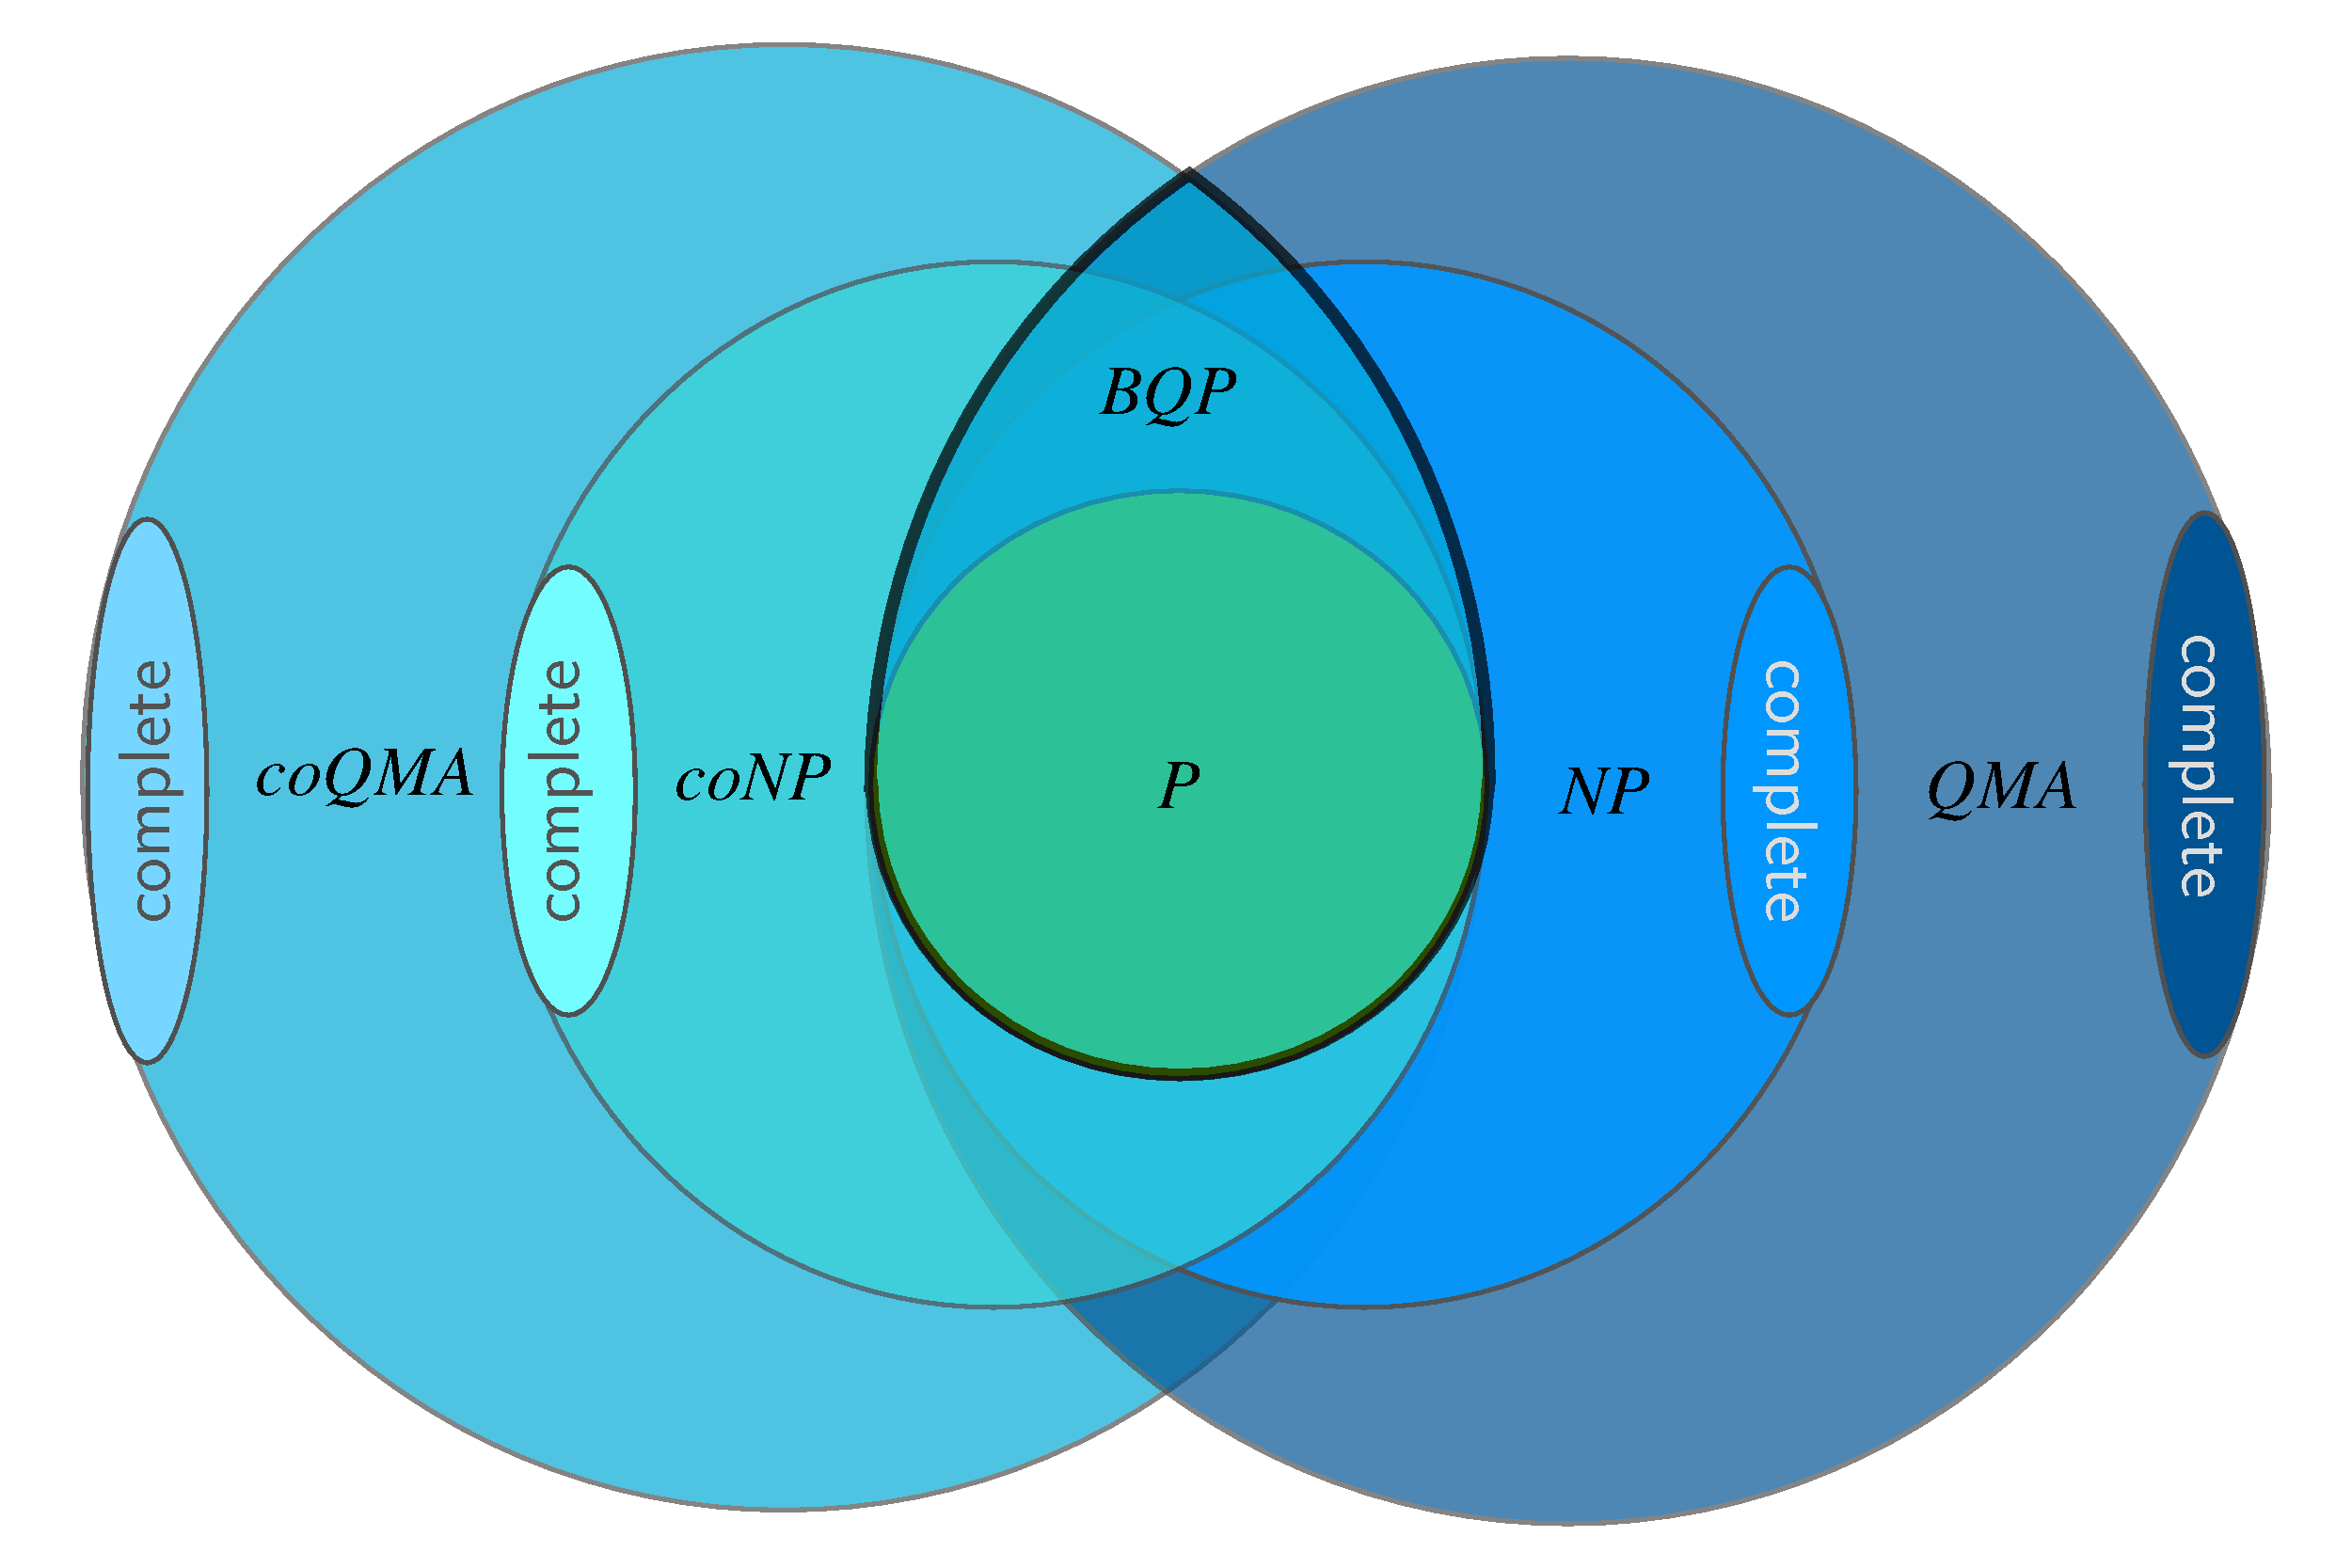
\includegraphics[width=0.85\linewidth]{src/complexity-classes-1.pdf}
		\caption{Complexity-Classes: Sketch of current assumptions. Known inclusions are: $\mathrm{P}\subseteq \mathrm{(co)NP} \subseteq \mathrm{(co)QMA}$ and $\mathrm{BQP}\subseteq \mathrm{(co)QMA}$. The rest of the sketch is conjectured but not proven.}
    \label{fig:complexity-classes}
\end{figure}

\begin{def*}[$\mathrm{QMA}$ Complete Problems] In the same way as for $\mathrm{NP}$-complete problems, we have $\mathrm{QMA}$ complete problems. Here, the most prominent one is the groundstate problem
\begin{align*}
    \texttt{GroundState} \in \mathrm{QMA}\text{-complete}
\end{align*}
\end{def*}
It turns out that not only is \texttt{GroundState} $\mathrm{QMA}$-complete, but also several restricted versions. It suffices for example to have a ``local'' Hamiltonian $H=\sum_i c_i h_i$, where the ``small'' Hamiltonians $h_i$ only act on a locally restricted part of the system -- in qubit language a $k$-local Hamiltonian can be represented like this, with all $h_i$ only acting on $k$ qubits of the total system.
For the $\mathrm{QMA}$ completeness it suffices to be 2-local, so these problems are already hard.

\subsection{Kitaev's Clock and QMA-Hardness} 
Here we will give an illustration about the main idea behind Kitaev's idea to show $\mathrm{QMA}$ hardness of \texttt{Groundstate}. We will try to focus on the key idea ommiting the nitty-gritty.\\

A quantum algorithm essentially works like this:
\begin{enumerate}
    \item prepare an initial basis state (or use the convention that we always start with $\ket{0}^N$
    \item apply a sequence of quantum gates $U_n\dots U_2U_1$
    \item read-out one (or multiple) qubits
\end{enumerate}
So the ``history'' of the computation is as follows
\begin{align}
    \ket{\psi_0} &= \ket{\mathbf{0}} \equiv \ket{0}^N\\
    \ket{\psi_1} &= U_1\ket{\psi_0}\\
    \vdots &\\
    \ket{\psi_i} &= U_i \ket{\psi_{i-1}} = U_i U_{i-1}\dots U_2U_1\ket{\psi_0}.
\end{align}
Going back to Feynman (and later Kitaev) we can define a ``history-state'' that contains all points of the computation
\begin{align}
    \ket{\Psi} = \frac{1}{\sqrt{n+1}}\left( \ket{\mathbf{0}}\otimes \ket{\mathbf{0}} + \sum_{k=1}^n \ket{\mathbf{k}} \otimes \ket{\psi_k} \right)
\end{align}
here, we added a second qubit register with $\lfloor \log_2(n)\rfloor + 1$ qubits that acts as an index for the individual epochs in the history of the computation.
We will now construct a Hamiltonian, such that the history state is it's groundstate with energy zero. This can be achieved as
\begin{align}
    H = H_0 + H_c +  H_n
\end{align}
using $H_0$ to ``fix'' the initial state, $H_c$ to encode the computation, and $H_n$ to encode the result. 
In our example, the initial state is supposed to be $\ket{\mathbf{0}}$, so we can just create a projector
\begin{align}
    H_0 = \ket{\mathbf{0}}\bra{\mathbf{0}} \otimes \left(1-\ket{\mathbf{0}}\bra{\mathbf{0}}\right)
\end{align}
so for the history state, we have
\begin{align}
    H_0 \ket{\Psi} = 0 \ket{\Psi}
\end{align}
and all other states with nonzero overlap with $\ket{\mathbf{0}}\otimes \ket{\psi}$ where $\braket{\mathbf{0}}{\psi}=0$ this will add a non-zero ``punishment''. This Hamiltonian alone does not distinguish between the history state and any other state that does not overlap with $\ket{\mathbf{0}}\otimes \ket{\psi}$ as given above. This is why the other two Hamiltonians are also needed. 
The computation can be encoded with 
\begin{align}
    H_c = \sum_{k=1}^{n-1} \ket{\mathbf{k}}\bra{\mathbf{k}}\otimes 1 + \ket{\mathbf{k}+1}\bra{\mathbf{k}+1}\otimes 1 - \ket{\mathbf{k}}\bra{\mathbf{k}+1} \otimes U^\dagger_{k} - \ket{\mathbf{k}+1}\bra{\mathbf{k}} \otimes U_{k}
\end{align}
because $U_k$ is the transition between the $k$th and $k+1$ step in the computation, while $U_k^\dagger$ is the inverse part. For the history state the two positive terms will cancel with the negative ones leading to an eigenvalue of zero.
In the end, we can also encode the desired output
\begin{align}
    H_n = \ket{\mathbf{n}}\bra{\mathbf{n}}\otimes P
\end{align}
where $P=\ket{0}\bra{0}\otimes 1\otimes 1\otimes \dots $ is a projector that adds a punishment if the circuit does not accept (i.e. if the designated output qubit is not in $\ket{1}$ at the end of the computation).\\

Through this construction we have the following equivalence: If the quantum algorithm $U_nU_{n-1}\dots U_2U_1\ket{0}$ accepts (i.e. the output qubit will be in $\ket{1}$) then the clock-Hamiltonian will have lowest eigenenergy zero and vice versa.\\

The previous illustration contains the main ideas that show the $\mathrm{QMA}$ hardness of \texttt{Groundstate}. Some comments to connect to the actual $\mathrm{QMA}$ hardness result
\begin{itemize}
    \item Instead of looking at a designated quantum algorithm that starts from $\ket{\mathbf0}$, we need to look at a quantum verifier -- a quantum circuit that can take an arbitrary $N$-qubit state (the certificate) as input. Essentially we just need to change $H_0$ (such that we do nothing on the input qubits that encode the quantum verifyier) for that.
    \item In order to show that local Hamiltonians (5-local in the original proof by Kitaev) we need to use a different encoding for the clock-register. Instead of $O(\log n)$ qubits, we can just use $n+1$ qubits and use unary encoding: $\ket{\mathbf{0}}=\ket{000\dots}, \ket{\mathbf{1}}=\ket{100\dots}, \ket{\mathbf{2}}=\ket{010\dots }, \ket{\mathbf{3}}=\ket{001\dots}$)
    \item $\mathrm{QMA}$ verification is probabilistic, i.e. it suffices if the circuit accepts with probability larger than 2/3 for a valid certificate. This needs to be considered. At the end you have something like: If there is a certificate such that the verifyier accepts with probability $1-\epsilon$, then the clock Hamiltonian has a groundstate close to zero, with some tolerance depending on $\epsilon$.
\end{itemize}
